%!Mode:: "TeX:UTF-8"
% 模板名称:UESTC_report
% 模板版本:V1.0(2019.12.12)
% 模板作者:SiYu Zhu
% 模板编译:XeLaTeX,如果要使用超链接\ref的话,编译两次,两次,两次!!!
% Github:https://github.com/zuicy/UESTC_report_latex
%
% 此模板为电子科技大学计算机学院实验报告模板,
% 是基于UESTC_Lab_Report_LaTeX_Template模板的改进版,
% 由于2019年下半学期实验中心更新了模板,因此对之前的模板进行了改进,
% 在此向这个模板的作者致谢!
% 主要改动有:
%           1.将配置单独放在了settings.tex文件中。
%           2.增加超链接跳转功能,方便图片与文字相隔很远时进行阅读。(默认为蓝色,
%           如需打印可在settings.tex中改为黑色或不使用超链接)
%           3.修改图表标题文字为五号。
%           4.更改模板样式为新版实验报告模板。
%           5.增加了代码选项列表。

\documentclass[a4paper,11pt,UTF8,AutoFakeBold= {2.88}]{ctexart}

\usepackage{indentfirst} %缩进
\usepackage{xeCJK}    %使用系统字体
\usepackage{fancyhdr} %自定义页眉页脚
\pagestyle{empty}                   %不设置页眉页脚
\usepackage{amsmath, amsthm, amssymb, amsfonts} %数学公式
\usepackage[a4paper,left=3cm,right=3cm,top=3cm,bottom=3cm]{geometry}
%\usepackage[tmargin=1in,bmargin=1in,lmargin=1.25in,rmargin=1.25in]{geometry}.
\usepackage{booktabs} %插入表格
\usepackage[section]{placeins} %避免浮动
\usepackage{listings} %插入代码
\usepackage{ctex}     %中文宏包
\usepackage[svgnames, table]{xcolor} %彩色表格
\usepackage{algorithm}          %伪代码
\usepackage{algorithmicx}
\usepackage{algpseudocode}
\usepackage{algorithm,algpseudocode,float}
\usepackage{lipsum}
\usepackage{enumitem}           %调整列举环境
\usepackage{fontspec,xunicode}
\defaultfontfeatures{Mapping=tex-text} %如果没有它,会有一些 tex 特殊字符无法正常使用,比如连字符。
\usepackage[colorlinks,linkcolor=blue,anchorcolor=blue,citecolor=blue,urlcolor=blue]{hyperref}
%超链接颜色配置,统一设置为了蓝色,如果希望可以跳转但不变颜色的话改为black


\usepackage{graphicx,subfig}
\graphicspath{{imgs/}}

%%%%%%%%%%%%%%%%%%%%%%%%%%%%%%%%%%%%%%%%%%%%%%%%%%%%%%%%%%%%%%%%
% 缩进及行间距
%%%%%%%%%%%%%%%%%%%%%%%%%%%%%%%%%%%%%%%%%%%%%%%%%%%%%%%%%%%%%%%%
\setlength{\parindent}{22pt} %重新定义缩进长度
\setlength{\baselineskip}{20pt}  %定义行间距
%\renewcommand{\baselinestretch}{1.1} %定义行间距

%%%%%%%%%%%%%%%%%%%%%%%%%%%%%%%%%%%%%%%%%%%%%%%%%%%%%%%%%%%%%%%%
% 列表设置
%%%%%%%%%%%%%%%%%%%%%%%%%%%%%%%%%%%%%%%%%%%%%%%%%%%%%%%%%%%%%%%%
\setenumerate{fullwidth,itemindent=\parindent,listparindent=\parindent,itemsep=0ex,partopsep=0pt,parsep=0ex}
\setenumerate[2]{label=\alph*),leftmargin=1.5em}  %二级item设置
\setitemize{itemindent=38pt,leftmargin=0pt,itemsep=-0.4ex,listparindent=26pt,partopsep=0pt,parsep=0.5ex,topsep=-0.25ex}
\setdescription{itemindent=38pt,leftmargin=0pt,itemsep=-0.4ex,listparindent=26pt,partopsep=0pt,parsep=0.5ex,topsep=-0.25ex}

%%%%%%%%%%%%%%%%%%%%%%%%%%%%%%%%%%%%%%%%%%%%%%%%%%%%%%%%%%%%%%%%
% 图的标题行间距设置
%%%%%%%%%%%%%%%%%%%%%%%%%%%%%%%%%%%%%%%%%%%%%%%%%%%%%%%%%%%%%%%%
\newcommand{\bottomcaption}{%
\setlength{\abovecaptionskip}{6pt}%
\setlength{\belowcaptionskip}{6pt}%
\caption}


%%%%%%%%%%%%%%%%%%%%%%%%%%%%%%%%%%%%%%%%%%%%%%%%%%%%%%%%%%%%%%%%
% 字体定义
%%%%%%%%%%%%%%%%%%%%%%%%%%%%%%%%%%%%%%%%%%%%%%%%%%%%%%%%%%%%%%%%
\setmainfont{Times New Roman}  %默认英文字体.serif是有衬线字体sans serif无衬线字体
\setmonofont{Consolas}
\setCJKmainfont[ItalicFont={楷体}, BoldFont={黑体}]{宋体}%衬线字体 缺省中文字体为
\setCJKsansfont{黑体}
\punctstyle{hangmobanjiao}
%-----------------------xeCJK下设置中文字体------------------------------%
\setCJKfamilyfont{song}{SimSun}                             %宋体 song
\newcommand{\song}{\CJKfamily{song}}
\setCJKfamilyfont{fs}{FangSong}                      %仿宋  fs
\newcommand{\fs}{\CJKfamily{fs}}
\setCJKfamilyfont{ktgb}{KaiTi}                      %楷体2312 ktgb
\newcommand{\ktgb}{\CJKfamily{ktgb}}
\setCJKfamilyfont{yh}{Microsoft YaHei}                    %微软雅黑 yh
\newcommand{\yh}{\CJKfamily{yh}}
\setCJKfamilyfont{hei}{SimHei}                              %黑体  hei
\newcommand{\hei}{\CJKfamily{hei}}
\setCJKfamilyfont{hwxk}{STXingkai}                                %华文行楷  hwxk
\newcommand{\hwxk}{\CJKfamily{hwxk}}
%------------------------------设置字体大小------------------------%
\newcommand{\shiyanbaogao}{\fontsize{36pt}{\baselineskip}\selectfont}
\newcommand{\chuhao}{\fontsize{44pt}{\baselineskip}\selectfont}     %初号
\newcommand{\xiaochuhao}{\fontsize{36pt}{\baselineskip}\selectfont} %小初号
\newcommand{\yihao}{\fontsize{26pt}{\baselineskip}\selectfont}      %一号
\newcommand{\xiaoyihao}{\fontsize{24pt}{\baselineskip}\selectfont}      %小一号
\newcommand{\erhao}{\fontsize{22pt}{\baselineskip}\selectfont}      %二号
\newcommand{\xiaoerhao}{\fontsize{18pt}{\baselineskip}\selectfont}  %小二号
\newcommand{\sanhao}{\fontsize{16pt}{\baselineskip}\selectfont}  %三号
\newcommand{\sihao}{\fontsize{14pt}{\baselineskip}\selectfont}       %四号
\newcommand{\xiaosihao}{\fontsize{12pt}{\baselineskip}\selectfont}  %小四号
\newcommand{\wuhao}{\fontsize{10.5pt}{\baselineskip}\selectfont}    %五号
\newcommand{\xiaowuhao}{\fontsize{9pt}{\baselineskip}\selectfont}   %小五号
\newcommand{\liuhao}{\fontsize{7.5pt}{\baselineskip}\selectfont}  %六号
\newcommand{\qihao}{\fontsize{5.5pt}{\baselineskip}\selectfont}    %七号

%%%%%%%%%%%%%%%%%%%%%%%%%%%%%%%%%%%%%%%%%%%%%%%%%%%%%%%%%%%%%%%%
% 图题字体大小相同
%%%%%%%%%%%%%%%%%%%%%%%%%%%%%%%%%%%%%%%%%%%%%%%%%%%%%%%%%%%%%%%%
\usepackage{caption}
\renewcommand{\small}{\wuhao}
\captionsetup{font={small}}   % small = 10.5pt
\captionsetup[lstlisting]{font={small}}

%%%%%%%%%%%%%%%%%%%%%%%%%%%%%%%%%%%%%%%%%%%%%%%%%%%%%%%%%%%%%%%%
% 重定义枚举编号为 1),2)...
%%%%%%%%%%%%%%%%%%%%%%%%%%%%%%%%%%%%%%%%%%%%%%%%%%%%%%%%%%%%%%%%
\renewcommand{\labelenumi}{\theenumi)}
\numberwithin{equation}{section}

%%%%%%%%%%%%%%%%%%%%%%%%%%%%%%%%%%%%%%%%%%%%%%%%%%%%%%%%%%%%%%%%
% 重定义section标题
%%%%%%%%%%%%%%%%%%%%%%%%%%%%%%%%%%%%%%%%%%%%%%%%%%%%%%%%%%%%%%%%
\CTEXsetup[format={\sihao\CJKfamily{SimSun}\zihao{4}},number={\textbf\chinese{section}},name={,、~},aftername={},indent={0pt},beforeskip={6pt},afterskip={6pt},format+={\flushleft\textbf}]{section}
\CTEXsetup[format={\Large\bfseries\CJKfamily{zhkai}\zihao{5}},name={(,)},number={\chinese{subsection}},aftername={},indent={22pt},beforeskip={14pt},afterskip={2pt}]{subsection}
\CTEXsetup[number={\chinese{section}},name={附录, ~~ }]{appendix}
%%%%%%%%%%%%%%%%%%%%%%%%%%%%%%%%%%%%%%%%%%%%%%%%%%%%%%%%%%%%%%%%
% 标题名称中文化
%%%%%%%%%%%%%%%%%%%%%%%%%%%%%%%%%%%%%%%%%%%%%%%%%%%%%%%%%%%%%%%%
\renewcommand\figurename{\hei 图}
\renewcommand\tablename{\hei 表}
\renewcommand\lstlistingname{\hei 代码}
\renewcommand{\algorithmicrequire}{\textbf{输入:}}
\renewcommand{\algorithmicensure}{\textbf{输出:}}
\newtheorem{define}{定义}
%%%%%%%%%%%%%%%%%%%%%%%%%%%%%%%%%%%%%%%%%%%%%%%%%%%%%%%%%%%%%%%%
% 代码设置
%%%%%%%%%%%%%%%%%%%%%%%%%%%%%%%%%%%%%%%%%%%%%%%%%%%%%%%%%%%%%%%%
\lstset{
 columns=fixed,
 numbers=left,                                        % 在左侧显示行号
 numberstyle=\tiny\color{gray},                       % 设定行号格式
 frame=single,                                        % 单线背景边框
 breaklines=true,                                     % 设定LaTeX对过长的代码行进行自动换行
 keywordstyle=\color[RGB]{40,40,255},                 % 设定关键字颜色
 numberstyle=\footnotesize\color{darkgray},
 commentstyle=\it\color[RGB]{0,96,96},                % 设置代码注释的格式
 stringstyle=\rmfamily\slshape\color[RGB]{128,0,0},   % 设置字符串格式
 showstringspaces=false,                              % 不显示字符串中的空格
% language=java,                                        % 设置语言
 basicstyle=\linespread{1.0}\xiaowuhao\ttfamily,                      % 字体字号
 %lineskip=10pt,
 %baselinestretch=1,
}

%%%%%%%%%%%%%%%%%%%%%%%%%%%%%%%%%%%%%%%%%%%%%%%%%%%%%%%%%%%%%%%%
% 伪代码分页
%%%%%%%%%%%%%%%%%%%%%%%%%%%%%%%%%%%%%%%%%%%%%%%%%%%%%%%%%%%%%%%%
\makeatletter
\renewcommand{\ALG@name}{算法}
\newenvironment{breakablealgorithm}
  {% \begin{breakablealgorithm}
   \begin{center}
     \refstepcounter{algorithm}% New algorithm
     \hrule height.8pt depth0pt \kern2pt% \@fs@pre for \@fs@ruled
     \renewcommand{\caption}[2][\relax]{% Make a new \caption
       {\raggedright\textbf{\ALG@name~\thealgorithm} ##2\par}%
       \ifx\relax##1\relax % #1 is \relax
         \addcontentsline{loa}{algorithm}{\protect\numberline{\thealgorithm}##2}%
       \else % #1 is not \relax
         \addcontentsline{loa}{algorithm}{\protect\numberline{\thealgorithm}##1}%
       \fi
       \kern2pt\hrule\kern2pt
     }
  }{% \end{breakablealgorithm}
     \kern2pt\hrule\relax% \@fs@post for \@fs@ruled
   \end{center}
  }
\makeatother



% 导入配置文件settings.tex,
% 配置参数均存储在settings.tex文件中,
% 添加或修改均需在该文件中进行

\begin{document}
\xiaosihao\song

\begin{titlepage}
      \leftline{\ktgb{\textbf{\yihao{ 电子科技大学}\underline{\xiaoyihao{计算机科学与工程学院}}}}}
\vspace{5.5cm}
\center{\shiyanbaogao{\ktgb{\textbf{标~ 准~ 实~ 验~ 报~ 告}}}}
\vspace{5.5cm}

\begin{center}
\begin{large}
\begin{tabular}{rc}

\xiaoerhao{\ktgb{\textbf{课程名称:}}}& \xiaoerhao{\ktgb{\textbf{互联网络程序设计}}}\\
\cline{2-2}\\
\xiaoerhao{\ktgb{\textbf{项目名称:}}}& \xiaoerhao{\ktgb{\textbf{非阻塞 DNS 客户端}}}\\
\cline{2-2}\\

\end{tabular}
\end{large}
\end{center}

\vspace{5cm}
\begin{center}
      \xiaosihao{\song{\textbf{电子科技大学教务处制表}}}
\end{center}

\end{titlepage}
\clearpage


\leftline{\\[10pt]\sihao{\textbf{\song{学生姓名:李有霖 \hfill 学号:202021080918 \hfill 指导教师:聂晓文}}}}

\setlength{\parskip}{6pt}  %定义段间距

\section{实验要求}

在一个 Reactor 网络库上采用非阻塞方式编写一个 DNS 客户端,获得 ip 地址:

\begin{enumerate}
      \item 查找资料了解 DNS 查询的报文交互过程,确定 RFC 对 DNS 交互报文的定义,根据报文定义设计并实现一个非阻塞 DNS 客户端
      \item 基于 Linux 平台,可以借助于 libuv 等现成网络库
\end{enumerate}

\section{实验原理}

\subsection{Domain Name System}


在 RFC1035 中定义了 DNS 的规范和实现,其中就包含对交互报文的定义。代码 \ref{message} 指出了报文的基本格式,其由五部分组成。Header节总是存在的,其指明了剩余的哪些节是存在的、此消息是请求还是响应和一些其他参数。

\begin{lstlisting}[label={message}, numbers=none,caption={DNS message format},captionpos=b]
      +---------------------+
      |        Header       |
      +---------------------+
      |       Question      | the question for the name server
      +---------------------+
      |        Answer       | RRs answering the question
      +---------------------+
      |      Authority      | RRs pointing toward an authority
      +---------------------+
      |      Additional     | RRs holding additional information
      +---------------------+
    \end{lstlisting}

代码 \ref{header} 是 Header 节的定义,由于我们只是实现域名到 ip 地址的转换,所以只需要关注一下几个域:

\begin{enumerate}
    \item ID:用于表示特定请求,由于我们实现的是非阻塞客户端,所以可能需要对不同请求设置不同的 ID。
    \item QDCOUNT:请求的域名数量。
    \item ANCOUNT:响应的域名数量。
\end{enumerate}

\begin{lstlisting}[label={header}, numbers=none,caption={Header section format}, captionpos=b]
      0  1  2  3  4  5  6  7  8  9  0  1  2  3  4  5
    +--+--+--+--+--+--+--+--+--+--+--+--+--+--+--+--+
    |                      ID                       |
    +--+--+--+--+--+--+--+--+--+--+--+--+--+--+--+--+
    |QR|   Opcode  |AA|TC|RD|RA|   Z    |   RCODE   |
    +--+--+--+--+--+--+--+--+--+--+--+--+--+--+--+--+
    |                    QDCOUNT                    |
    +--+--+--+--+--+--+--+--+--+--+--+--+--+--+--+--+
    |                    ANCOUNT                    |
    +--+--+--+--+--+--+--+--+--+--+--+--+--+--+--+--+
    |                    NSCOUNT                    |
    +--+--+--+--+--+--+--+--+--+--+--+--+--+--+--+--+
    |                    ARCOUNT                    |
    +--+--+--+--+--+--+--+--+--+--+--+--+--+--+--+--+
\end{lstlisting}

代码 \ref{ques} 是 Question 节的格式,当 QDCOUNT 不为 0 时其存放具体的请求。QNAME 域变长,存放请求的域名字符串,这里使用了一种压缩的存储方式,就不在此具体介绍了。QTYPE 存放请求的类型,在本例中类型均为 A。QCLASS 指定查询类,在本例中恒为 IN。

\begin{lstlisting}[label={ques}, numbers=none,caption={Question section format}, captionpos=b]
    0  1  2  3  4  5  6  7  8  9  0  1  2  3  4  5
    +--+--+--+--+--+--+--+--+--+--+--+--+--+--+--+--+
    |                                               |
    /                     QNAME                     /
    /                                               /
    +--+--+--+--+--+--+--+--+--+--+--+--+--+--+--+--+
    |                     QTYPE                     |
    +--+--+--+--+--+--+--+--+--+--+--+--+--+--+--+--+
    |                     QCLASS                    |
    +--+--+--+--+--+--+--+--+--+--+--+--+--+--+--+--+
\end{lstlisting}

代码 \ref{respon} 是 DNS 服务器响应的格式,在本例中只关心 RDATA 域,当请求是 A 时,其为 4 字节数据,存储了查询到的 ip 地址。

\begin{lstlisting}[label={respon}, numbers=none,caption={Resource record format}, captionpos=b]
    0  1  2  3  4  5  6  7  8  9  0  1  2  3  4  5
    +--+--+--+--+--+--+--+--+--+--+--+--+--+--+--+--+
    |                                               |
    /                                               /
    /                      NAME                     /
    |                                               |
    +--+--+--+--+--+--+--+--+--+--+--+--+--+--+--+--+
    |                      TYPE                     |
    +--+--+--+--+--+--+--+--+--+--+--+--+--+--+--+--+
    |                     CLASS                     |
    +--+--+--+--+--+--+--+--+--+--+--+--+--+--+--+--+
    |                      TTL                      |
    |                                               |
    +--+--+--+--+--+--+--+--+--+--+--+--+--+--+--+--+
    |                   RDLENGTH                    |
    +--+--+--+--+--+--+--+--+--+--+--+--+--+--+--+--|
    /                     RDATA                     /
    /                                               /
    +--+--+--+--+--+--+--+--+--+--+--+--+--+--+--+--+
\end{lstlisting}

\subsection{Unicorn Velociraptor}

libuv库是多平台C库,提供对基于事件循环的异步I/O的支持。它支持epoll、kqueue、Windows的IOCP和Solaris的事件端口。它主要设计用于Node.js,但也可用于其他软件项目如Julia或pyuv等。它最初是libev或Microsoft IOCP上的抽象,libev只支持Unix系统而不支持Windows上的IOCP,在node-v0.9.0的libuv版本中去除了对libev的依赖。

\section{实验步骤}

\subsection{总体架构设计}

由于实现一个非阻塞的客户端,理所应当需要接受用户多个输入。所以在 libuv 事件循环中绑定标准输入并且设置 read 回调函数。实现 DNS 客户端需要以 udp 的方式创建一个 socket,并在事件循环中绑定,并设置 recv 回调函数。总体执行流程如图 \ref{timeline} 所示,libuv 接受到用户输入时调用 read 回调函数,其将会根据用户的输入构建 DNS 请求报文发送给 DNS 服务器。DNS 服务器在查询结束后响应,libuv 接收到服务器的响应报文后调用 recv 回调函数,从报文中提取出 ip 地址并输出。

\begin{figure}[!htbp]
    \centering
    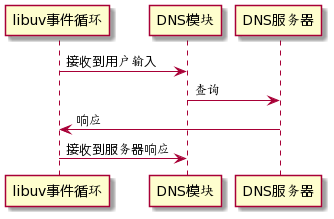
\includegraphics[scale=0.8]{timeline}
    \bottomcaption{\wuhao{程序执行流程}}
    \label{timeline}
    \end{figure}

\subsection{DNS 模块的设计与实现}

DNS 模块的核心代码就是根据用户请求的域名构建请求报文,和从服务器的响应报文中提取出 ip 信息。有了实验原理章节的介绍,已经对报文结构有了足够的理解,接下来就是编写代码实现具体功能。

代码 \ref{make-req} 是构造请求报文的主要代码:13-19 行构造报文的 Header 节,赋值 id、将 qcount 域设置为 1,表示本次请求只包含一个域名;21-38 行构造报文的 Question 节,首先根据压缩算法写入请求的域名,然后设置 QTYPE 和 QCLASS 域。

\begin{lstlisting}[label={make-req}, caption={构造请求报文}, captionpos=b, language=c]
uv_buf_t make_dns_query_msg(char *host_name, ssize_t len_host_name){
    for(int i=0; i<len_host_name; i++){
        if(host_name[i] == '\n'){
            host_name[i] = '\0';
        }
    }
    char *buf = (char *)malloc(MAX_DNS_PACKAGE_SIZE);
    memset((void *)buf, 0, MAX_DNS_PACKAGE_SIZE);

    DNS_HEADER *dns_hdr = (DNS_HEADER *)buf;
    int id = get_dns_id(host_name);

    printf("[+] Query for {%d}%s\n", id, host_name);
    dns_hdr->id = htons(id);
    dns_hdr->rd = 1;
    dns_hdr->qcount = htons(1);
    dns_hdr->ancount = htons(0);
    dns_hdr->nscount = htons(0);
    dns_hdr->arcount = htons(0);

    strcpy(buf + sizeof(DNS_HEADER)+1, host_name);
    char *p = buf+sizeof(DNS_HEADER)+1;
    u_char i = 0;
    while (p < buf+sizeof(DNS_HEADER)+strlen(host_name)+1){
        if(*p == '.'){
            p[-i-1] = i;
            i = 0;
        }
        else{
            i++;
        }
        p++;
    }
    p[-i-1] = i;

    DNS_QUESTION_SECTION_TAIL *dns_tail = (DNS_QUESTION_SECTION_TAIL *)(p+1);
    dns_tail->qtype = htons(DNS_QTYPE_A);
    dns_tail->qclass = htons(DNS_QCLASS_IN);

    return uv_buf_init(buf, sizeof(DNS_HEADER)+sizeof(DNS_QUESTION_SECTION_TAIL)\
            +strlen(host_name)+2);
}
\end{lstlisting}

代码 \ref{parse-res} 是接收到响应报文的回调函数,其主要负责解析响应报文,并输出查询结果:11 行首先获得报文的 id 域的数据,用来查找该报文对应请求的域名;14-16 行从报文中读取 RDATA 域的数据,并将查询结果输出。

\begin{lstlisting}[label={parse-res},caption={解析响应报文},captionpos=b,language=c]
void on_dns_read(uv_udp_t *req, ssize_t nread, const uv_buf_t *buf,\
        const struct sockaddr *addr, unsigned flags){
    if(nread < 0){
        fprintf(stderr, "Read error %s\n", uv_err_name(nread));
        uv_close((uv_handle_t *)req, NULL);
        free(buf->base);
        return;
    }
    else if(nread > 0){
        DNS_HEADER *header = (DNS_HEADER *)buf->base;
        u_int id = ntohs(header->id);
        char *host_name = get_dns_host_name(id);
        if (header->ancount){
            u_char *rdata = (u_char *)(buf->base+nread-4);
            printf("[*] {%u}%s -> %u.%u.%u.%u\n", id, host_name, rdata[0], rdata[1],\
                    rdata[2], rdata[3]);
        }
        else{
            printf("[-] {%u}DNS query failed for %s\n", id, host_name);
        }
        // Free the chunk allocated by alloc_stdin_bufffer
        free(host_name);
    }
    free(buf->base);
    return;
}
\end{lstlisting}

\section{实验数据及结果与分析}

图 \ref{exp} 是程序运行时的截图,我们首先查询 baidu.com,可以发现程序很好的发送了请求并且解析了服务器的响应。接着查询 k1ll3r.io,可能由于缓存没有命中,该次查询没有立即返回。紧接着我们查询 cnss.io ,程序同样很好的处理了请求并解析了结果。可以发现由于上一次请求没有返回,这一次报文的 id 域的数值增加了,很好的处理了非阻塞的情况,也很好的体现了程序非阻塞的特性。

\begin{figure}[!htbp]
    \centering
    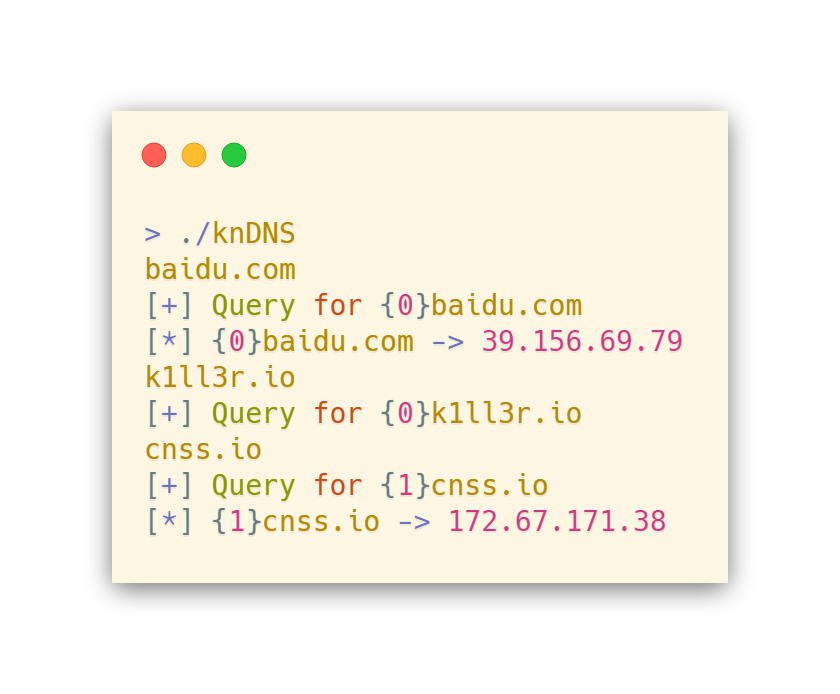
\includegraphics[scale=0.4]{exp}
    \bottomcaption{\wuhao{程序运行截图}}
    \label{exp}
    \end{figure}

\section{实验结论、心得体会}

借此实验很好地学习了网络程序设计的知识,包括很多报告中没有体现的基础知识,例如 TCP/IP 协议的细节、IO 复用编程、多进程多线程并发等等。也深刻地体会到了实现一个能很好处理并发的网络程序的不易。

\vspace{4cm}
\begin{flushright}
\begin{tabular}{lc}
\sihao{\song{\textbf{报告评分:}}}& \sihao{\textbf{\song{}}}\\
\sihao{\song{\textbf{指导教师签字:}}}& \sihao{\song{\textbf{}}}\\
\end{tabular}
\end{flushright}

\end{document}
